\documentclass[aspectratio=169]{beamer}
\usepackage{tikz}

\begin{document}
\begin{frame}{MTH 1020 Week 6 tutorial}
\begin{enumerate}
  \item Some reminders on geometry of complex numbers
  \item Fractals
\end{enumerate}
\end{frame}

\begin{frame}{Definition of complex numbers}

\begin{definition}
A \textbf{complex number} is a sum $ x + y i $ where $ x, y \in \mathbb{R} $ and where $ i $ is a symbol satisfying $ i^2 = -1 $.
\end{definition}

\begin{example}
  If $ z = 2 + 3i $ then
  \begin{align*}
    z^2 + z + 1 &= (2 + 3i)^2 + (2+2i) + 1\\
                &= (4 + 12i + 9i^2) + (2+2i) + 1\\
                &= (4 + 12i - 9) + (2+2i) + 1\\
                &= -2 + 14i.
  \end{align*}
\end{example}

Hurwitz (1923) showed that there are only 3 possible ways to extend the real numbers by adding new symbols to get a system of numbers which still has an absolute value:
the complex numbers (2D), the \textbf{quaternions} (4D), and the \textbf{octonions} (8D).

\end{frame}

\begin{frame}{Argand diagram}

\begin{columns}
\begin{column}{.4\textwidth}
\begin{itemize}
  \item Since $ i^4 = (i^2)^2 = 1 $, it is natural to think about multiplication by $ i $ as some kind of rotation by an angle $ 2\pi/4 = 90^\circ $.
  \item So $ 4i $ should be the number obtained by rotating $ 4 $ by $ 90^\circ $.
\end{itemize}

\end{column}
\begin{column}{.6\textwidth}
\begin{tikzpicture}[scale=.8]
    \begin{scope}[thick,font=\scriptsize]


    \draw [->] (-4,0) -- (4,0) node [above left]  {$\Re z$};
    \draw [->] (0,-4) -- (0,4) node [below right] {$\Im z$};


    \foreach \n in {-3,...,-1,1,2,...,3}{%
        \draw (\n,-3pt) -- (\n,3pt)   node [above] {$\n$};
        \draw (-3pt,\n) -- (3pt,\n)   node [right] {$\n i$};}

    \draw [thick, color=red] (0,0) -- (2,3);
    \draw [color=blue, fill=blue] (2,3) circle(0.05);
    \node [color=black] at (3,3) {$ 2+3i$};
\end{scope}
\end{tikzpicture}
\end{column}
\end{columns}

\end{frame}

\begin{frame}{Geometric meaning of complex numbers}

\begin{itemize}
  \item Complex numbers \emph{add} like vectors, easiest in rectangular form.
  \item Complex numbers \emph{multiply} by rotating and scaling, easiest in polar form.
\end{itemize}

All the geometry that you can do is shifts, and rotating and scaling.

\end{frame}

\begin{frame}{While we are thinking geometrically...}

Here are two functions:

\begin{displaymath}
  f(z) = z + 1 \text{ and } g(z) = \frac{z}{2i \cdot z + 1}.
\end{displaymath}
We will make a list of numbers $ z_1, z_2, ... $.
\begin{enumerate}
  \item  Take $ z_1 = 0 $.
  \item To produce point $ z_n $:
  \begin{enumerate}
    \item Randomly choose $ f $, $ f^{-1} $, $ g $, or $ g^{-1} $.
    \item Apply the function you just chose to $ z_{n-1} $; so you randomly have
      \begin{gather*}
        z_n = f(z_{n+1}) \text{ or } z_n = g(z_{n+1}) \text{ or}\\
        z_n = f^{-1}(z_{n+1}) \text{ or } z_n = g^{-1}(z_{n+1})
      \end{gather*}
  \end{enumerate}
  \item Plot all the points on an Argand diagram.
\end{enumerate}

\end{frame}

\begin{frame}{While we are thinking geometrically...}
\begin{columns}
\begin{column}{.5\textwidth}
\begin{displaymath}
  f(z) = z + 1 \text{ and } g(z) = \frac{z}{2i \cdot z + 1}.
\end{displaymath}
We will make a list of numbers $ z_1, z_2, ... $.
\begin{enumerate}
  \item Take $ z_1 = 0 $.
  \item To produce point $ z_n $:
  \begin{enumerate}
    \item Randomly choose $ f $, $ f^{-1} $, $ g $, or $ g^{-1} $.
    \item Apply the function you just chose to $ z_{n-1} $; so you randomly have
      \begin{gather*}
        z_n = f(z_{n+1}) \text{ or } z_n = g(z_{n+1}) \text{ or}\\
        z_n = f^{-1}(z_{n+1}) \text{ or } z_n = g^{-1}(z_{n+1})
      \end{gather*}
  \end{enumerate}
  \item Plot all the points on an Argand diagram.
\end{enumerate}
\end{column}
\begin{column}{.5\textwidth}
\begin{overprint}
\includegraphics<1>[width=\textwidth]{plot_0}
\includegraphics<2>[width=\textwidth]{plot_1}
\includegraphics<3>[width=\textwidth]{plot_1b}
\includegraphics<4>[width=\textwidth]{plot_2}
\includegraphics<5>[width=\textwidth]{plot_2b}
\includegraphics<6>[width=\textwidth]{plot_3}
\includegraphics<7>[width=\textwidth]{plot_4}
\includegraphics<8>[width=\textwidth]{plot_5}
\includegraphics<9>[width=\textwidth]{plot_6}
\end{overprint}
\end{column}
\end{columns}
\end{frame}

\begin{frame}
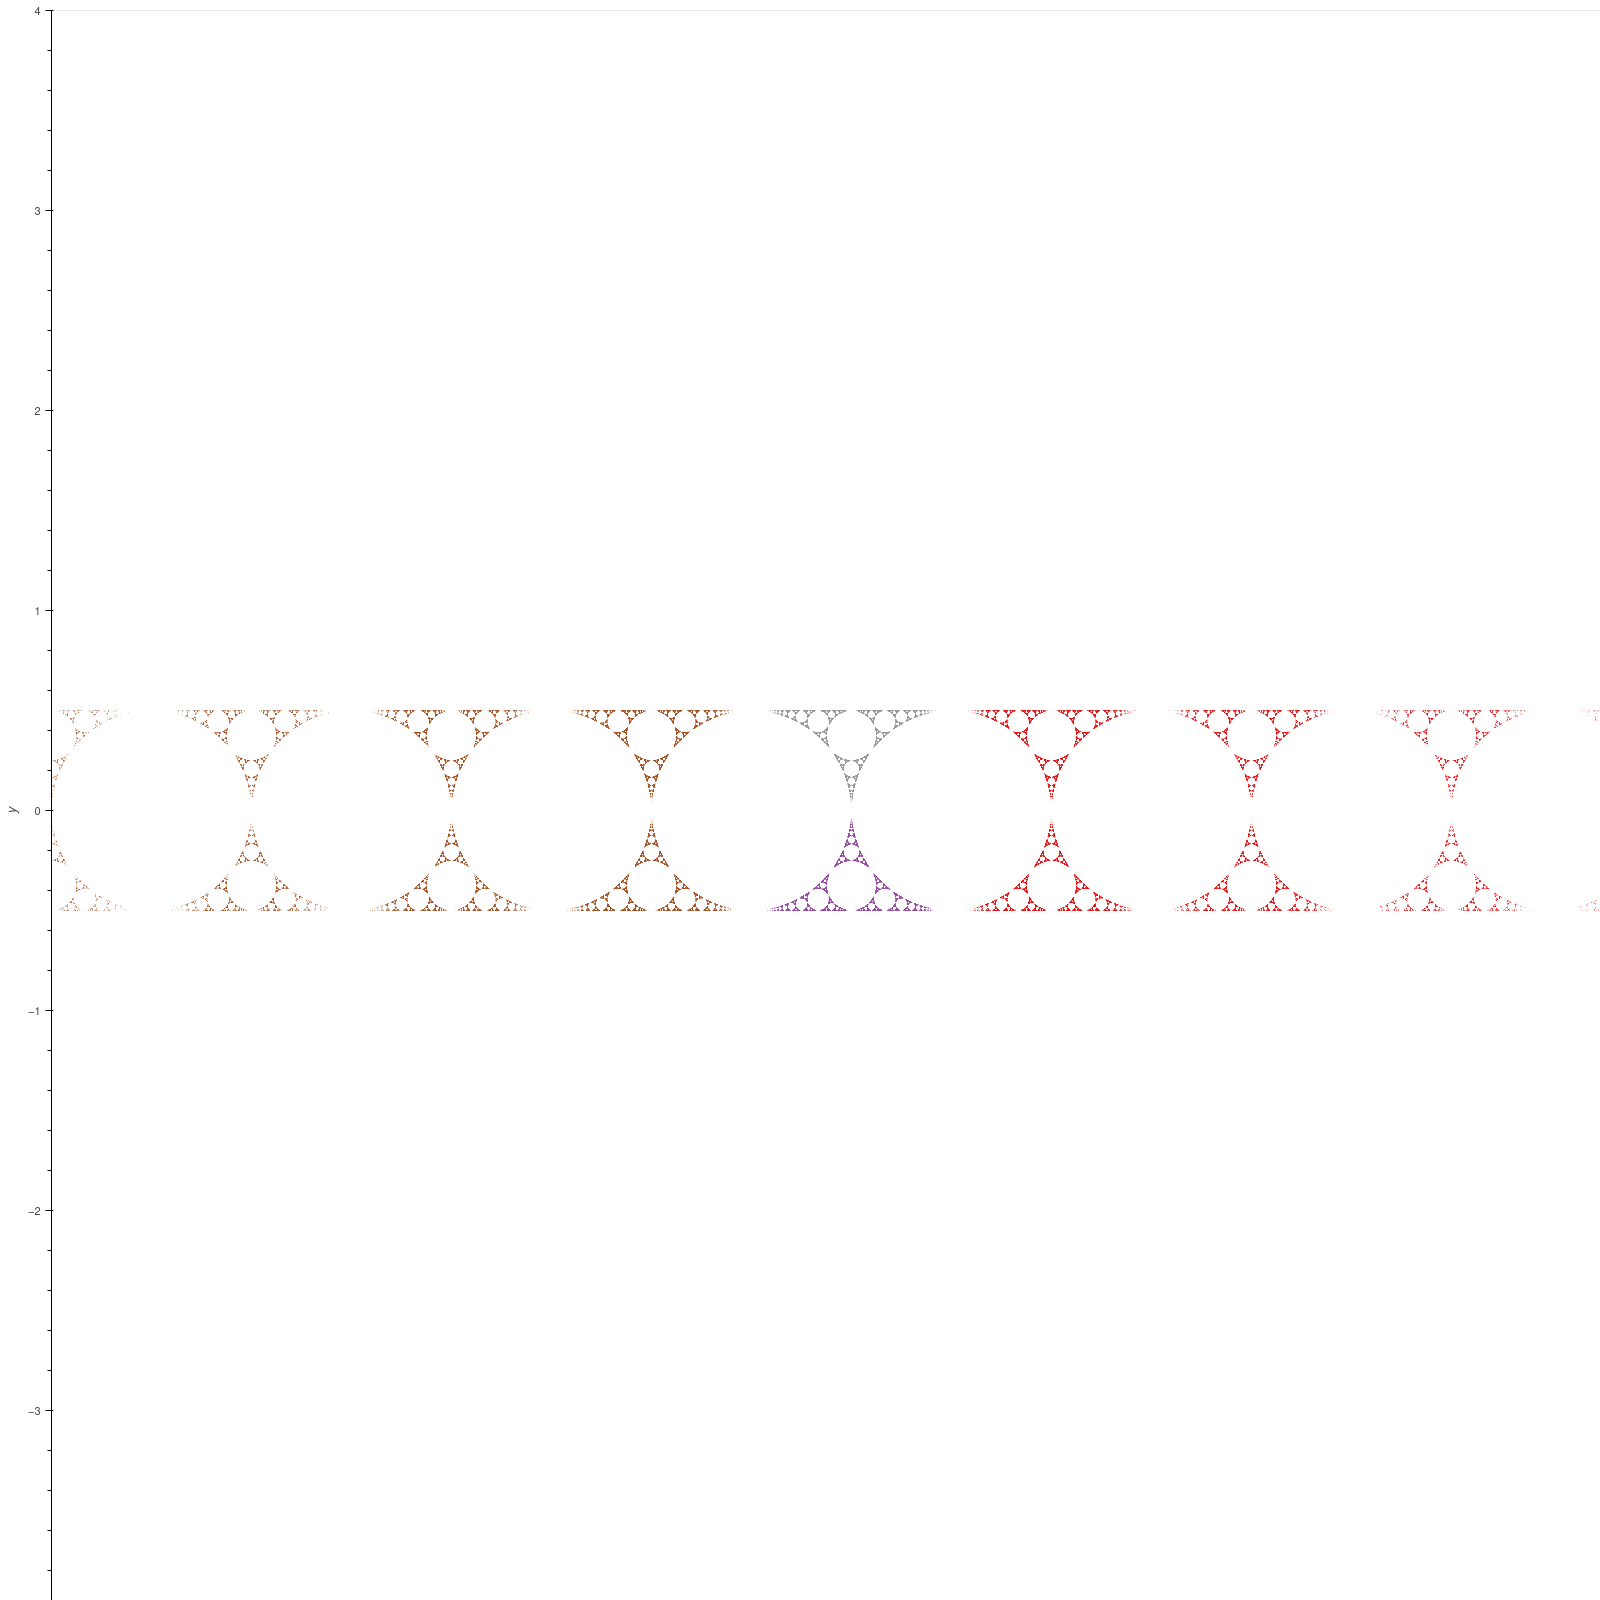
\includegraphics[width=\textwidth]{../../zoo/apollonian_gasket.png}
This is a fractal called the \textbf{Apollonian gasket}. We just make it by writing down a list of complex numbers one after another,
following a simple arithmetic rule at each step.
\end{frame}

\begin{frame}
\includegraphics[width=.33\textwidth]{../../zoo/bianchi_O2.png}%
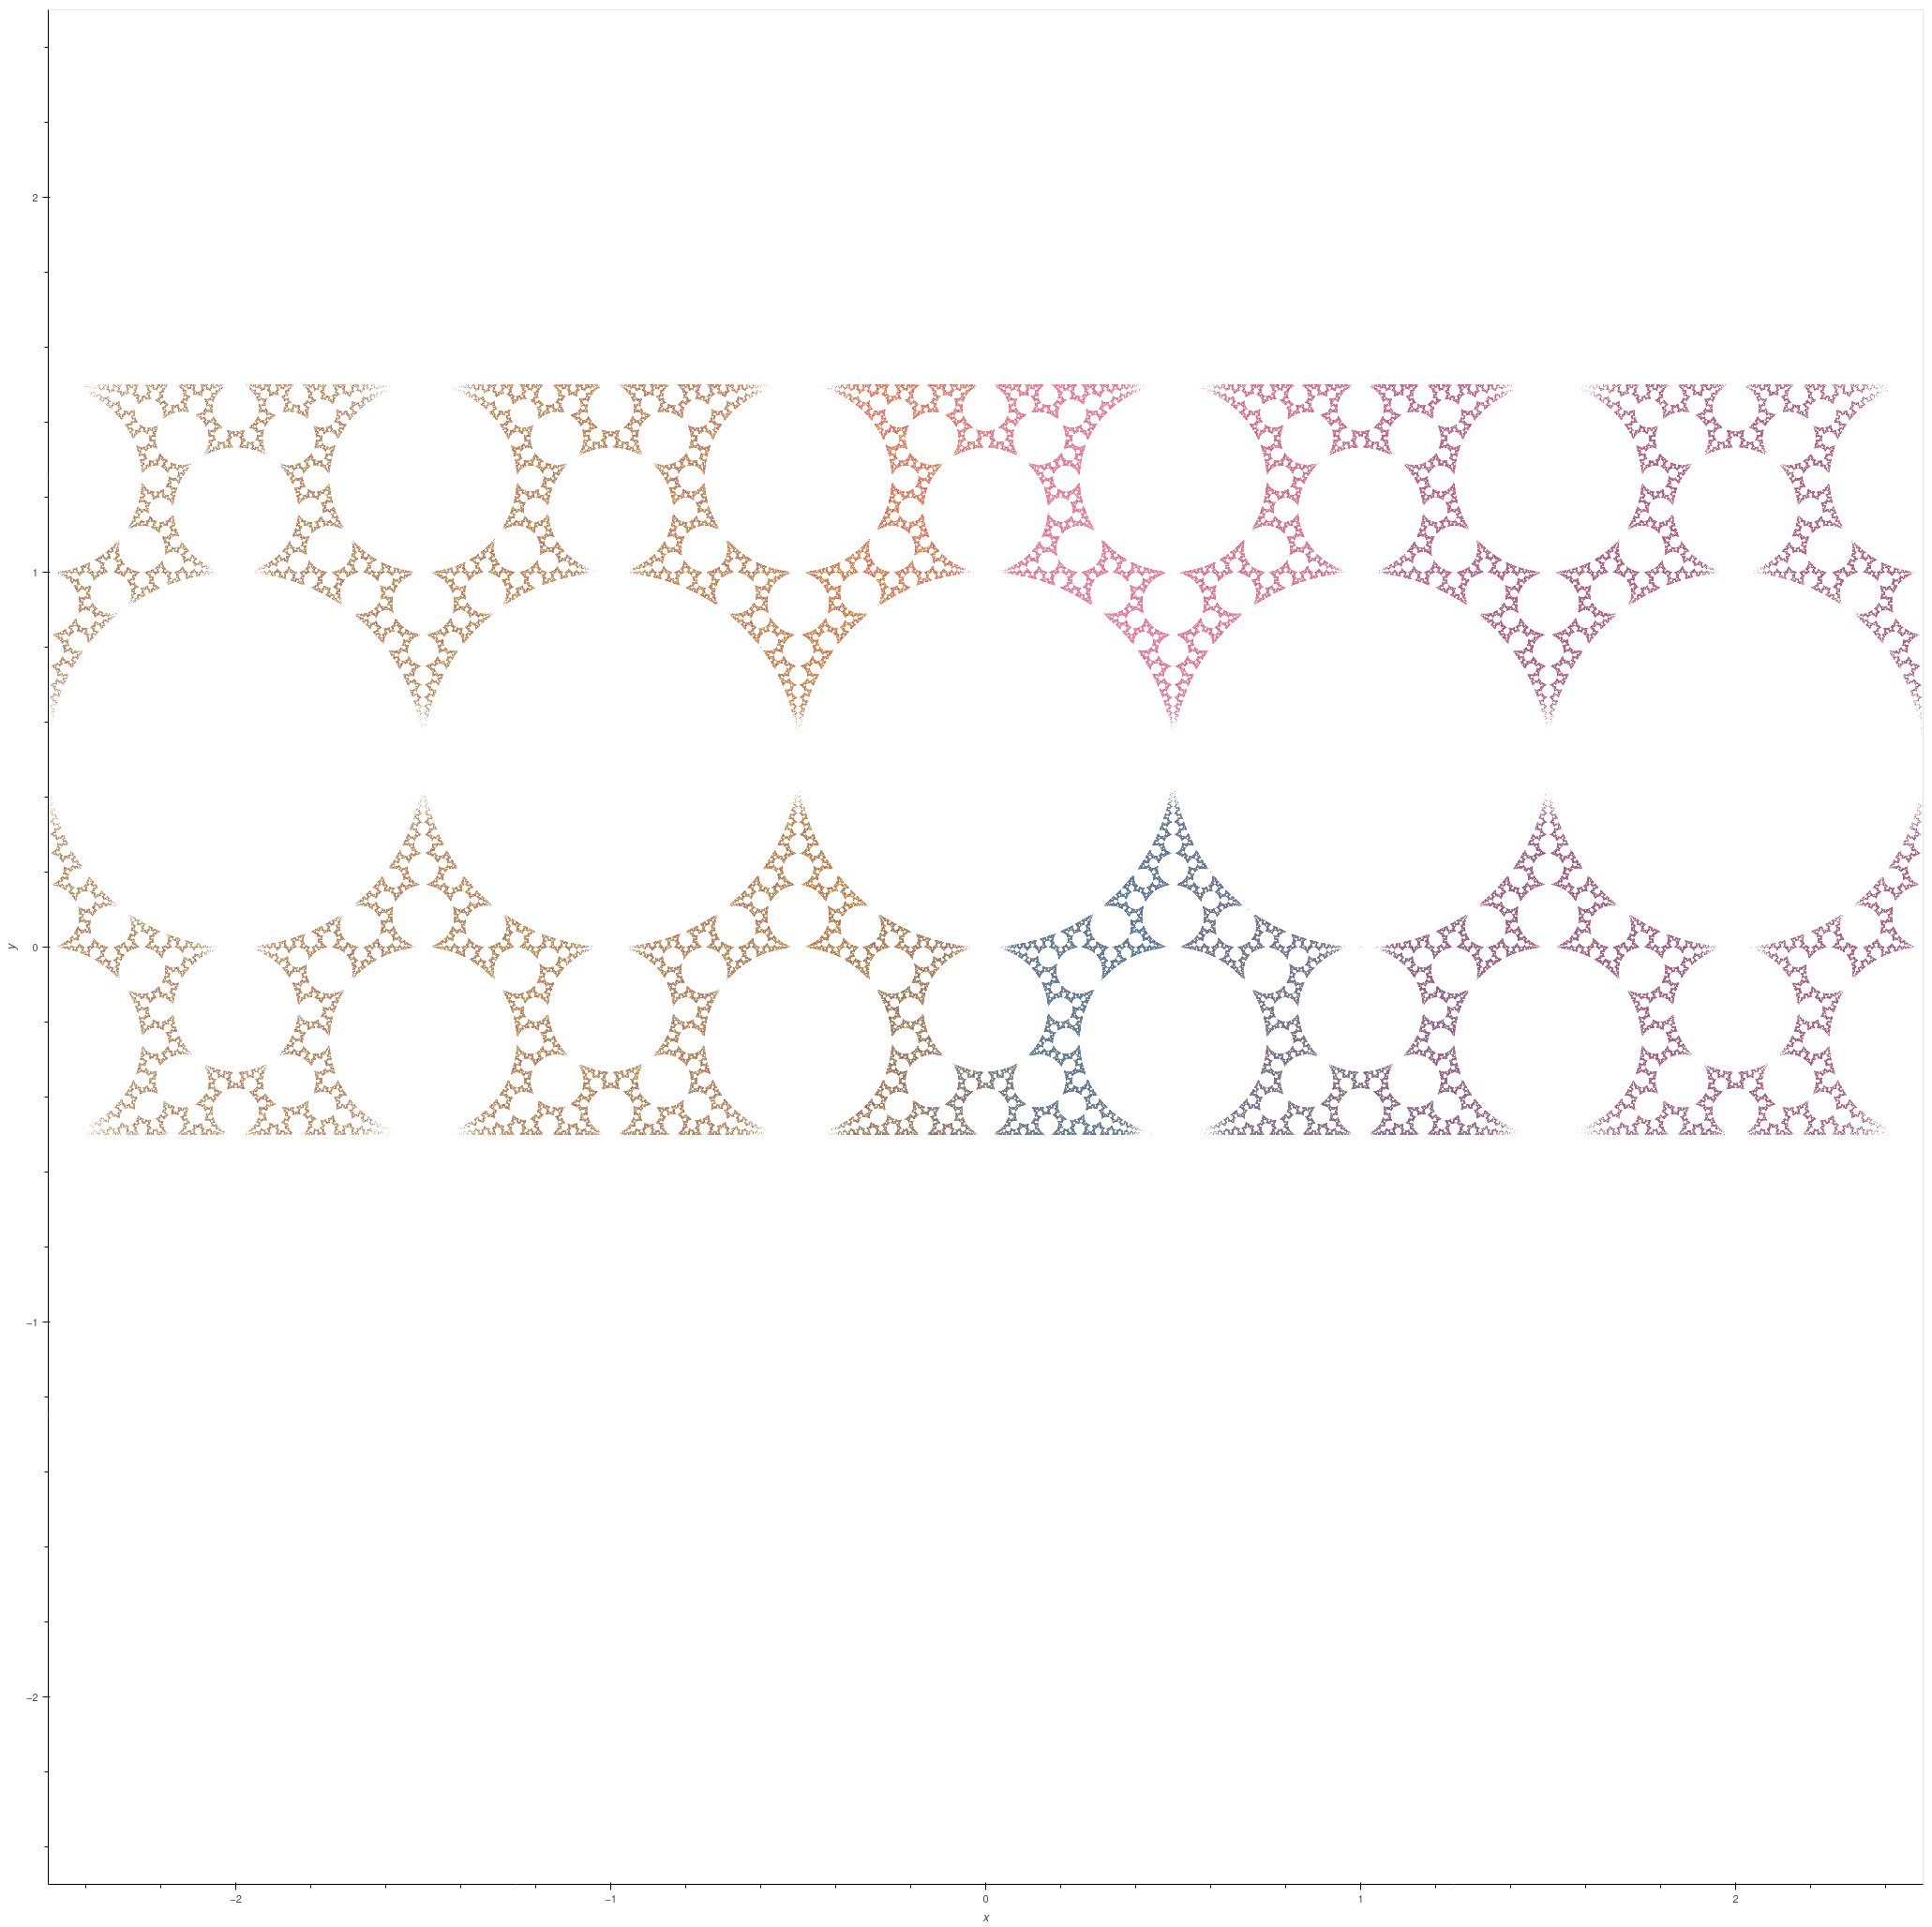
\includegraphics[width=.33\textwidth]{../../zoo/modular_group_1.png}%
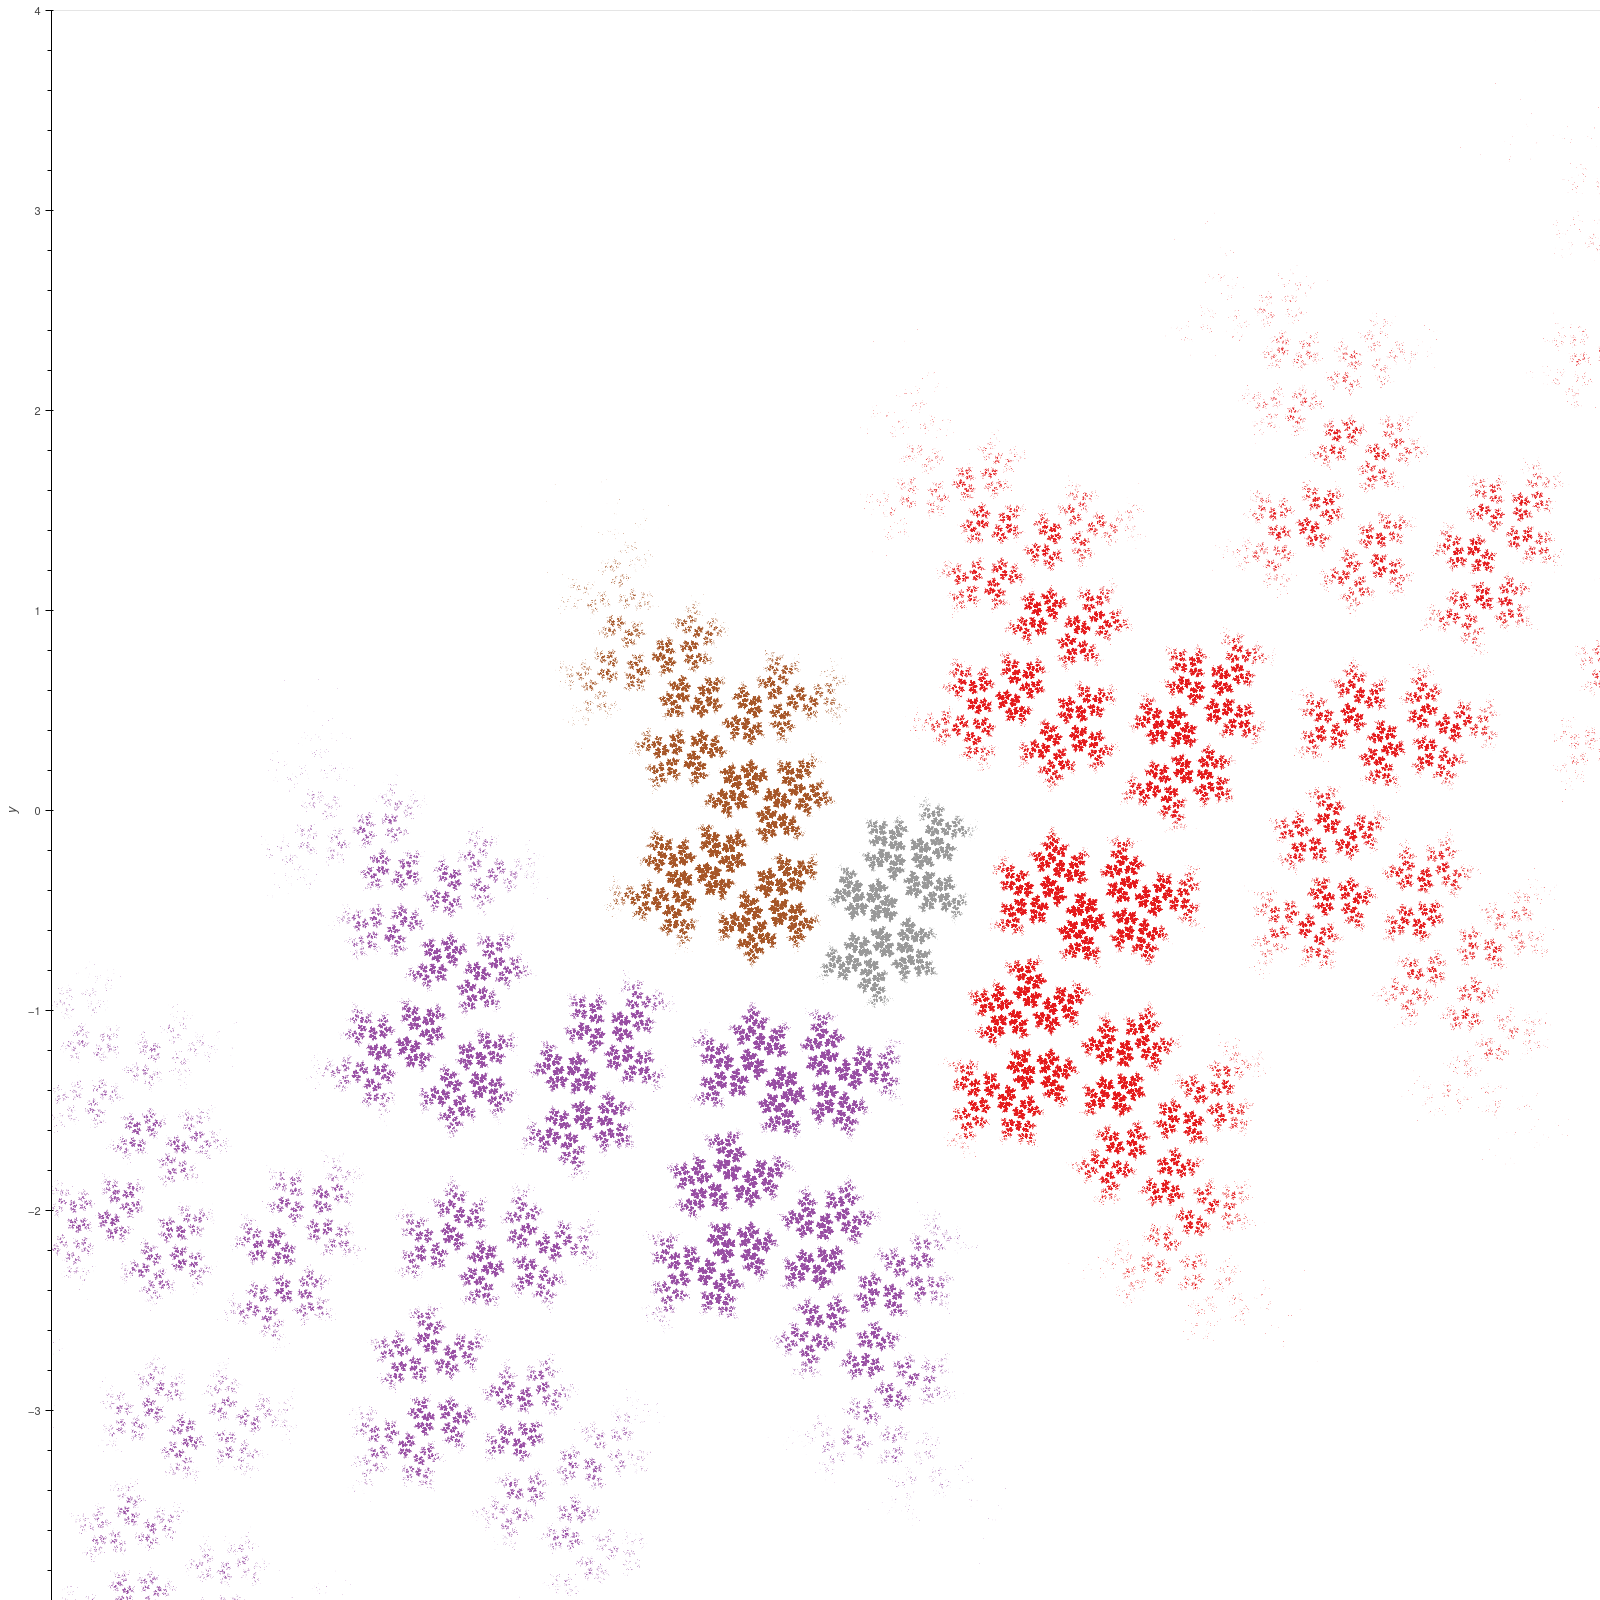
\includegraphics[width=.33\textwidth]{../../zoo/jorgensen_marden1.png}\\
Three other fractals you can make in the same way (just different randomly chosen functions. These are called \textbf{Kleinian fractals}. Other kinds of fractals
you can get from the complex numbers are \textbf{Julia sets} and the \textbf{Mandelbrot set}. There are nice animations on YouTube. It is all just arithmetic of complex numbers.
\end{frame}

\begin{frame}{MTH 1020 Week 5 tutorial}
\begin{enumerate}
  \item Get into groups of 3-4 people who all prepared a different question in advance.
  \item Write your \textbf{preferred name} and \textbf{ID number} on the whiteboards so I can take attendance
  \item Present your prepared question to each other as I come around, you should only take about 5min each for this.
  \item Then get started on the other questions \textbf{in your groups}.
  \item \textbf{At the end:} please erase the boards and return any markers etc that you used (you do not need to return the handouts)
\end{enumerate}
\end{frame}



\end{document}
